% Chapter 7: Cointegration and VECM
% Harvard-quality academic presentation
% Bachelor program, Bucharest University of Economic Studies

\documentclass[9pt, aspectratio=169, t]{beamer}

% Ensure content fits on slides
\setbeamersize{text margin left=8mm, text margin right=8mm}

%=============================================================================
% THEME AND STYLE CONFIGURATION
%=============================================================================
\usetheme{default}
% Using default theme for clean header/footer control

% Color Palette (matching Redispatch PDF)
\definecolor{MainBlue}{RGB}{26, 58, 110}
\definecolor{AccentBlue}{RGB}{26, 58, 110}
\definecolor{IDAred}{RGB}{205, 0, 0}
\definecolor{DarkGray}{RGB}{51, 51, 51}
\definecolor{MediumGray}{RGB}{128, 128, 128}
\definecolor{LightGray}{RGB}{248, 248, 248}
\definecolor{VeryLightGray}{RGB}{235, 235, 235}
\definecolor{KeynoteGray}{RGB}{218, 218, 218}
\definecolor{SectionGray}{RGB}{120, 120, 120}
\definecolor{FooterGray}{RGB}{100, 100, 100}
\definecolor{Crimson}{RGB}{220, 53, 69}
\definecolor{Forest}{RGB}{46, 125, 50}
\definecolor{Amber}{RGB}{181, 133, 63}
\definecolor{Orange}{RGB}{230, 126, 34}
\definecolor{Purple}{RGB}{142, 68, 173}

% Gradient background (exact Keynote 315° gradient: white to RGB 218,218,218)
\setbeamertemplate{background}{%
    \begin{tikzpicture}[remember picture, overlay]
        \shade[shading=axis, shading angle=315,
        top color=white, bottom color=KeynoteGray]
        (current page.south west) rectangle (current page.north east);
    \end{tikzpicture}%
}
% Fallback solid color for compatibility
\setbeamercolor{background canvas}{bg=}

\setbeamercolor{palette primary}{bg=MainBlue, fg=white}
\setbeamercolor{palette secondary}{bg=MainBlue!85, fg=white}
\setbeamercolor{palette tertiary}{bg=MainBlue!70, fg=white}
\setbeamercolor{structure}{fg=MainBlue}
\setbeamercolor{title}{fg=IDAred}
\setbeamercolor{frametitle}{fg=IDAred, bg=}
\setbeamercolor{block title}{bg=MainBlue, fg=white}
\setbeamercolor{block body}{bg=VeryLightGray, fg=DarkGray}
\setbeamercolor{block title alerted}{bg=Crimson, fg=white}
\setbeamercolor{block body alerted}{bg=Crimson!8, fg=DarkGray}
\setbeamercolor{block title example}{bg=Forest, fg=white}
\setbeamercolor{block body example}{bg=Forest!8, fg=DarkGray}
\setbeamercolor{item}{fg=MainBlue}

% Footer colors (override Madrid theme blue)
\setbeamercolor{author in head/foot}{fg=FooterGray, bg=}
\setbeamercolor{title in head/foot}{fg=FooterGray, bg=}
\setbeamercolor{date in head/foot}{fg=FooterGray, bg=}
\setbeamercolor{section in head/foot}{fg=FooterGray, bg=}
\setbeamercolor{subsection in head/foot}{fg=FooterGray, bg=}

% Bullet styles (apply everywhere including blocks)
\setbeamertemplate{itemize item}{\color{MainBlue}$\boxdot$}
\setbeamertemplate{itemize subitem}{\color{MainBlue}$\blacktriangleright$}
\setbeamertemplate{itemize subsubitem}{\color{MainBlue}\tiny$\bullet$}
\setbeamertemplate{itemize/enumerate body begin}{\normalsize}
\setbeamertemplate{itemize/enumerate subbody begin}{\normalsize}

% Item spacing - compact style
\setlength{\leftmargini}{10pt}       % Level 1: minimal indent
\setlength{\leftmarginii}{10pt}      % Level 2: minimal additional indent
% Compact list spacing (zero extra space before/after lists in blocks)
\makeatletter
\def\@listi{\leftmargin\leftmargini \topsep 0pt \parsep 0pt \itemsep 0pt}
\def\@listii{\leftmargin\leftmarginii \topsep 0pt \parsep 0pt \itemsep 0pt}
\makeatother

\setbeamertemplate{navigation symbols}{}

%=============================================================================
% CUSTOM HEADLINE
%=============================================================================
\setbeamertemplate{headline}{%
    \vskip10pt%
    \hbox to \paperwidth{%
        \hskip0.5cm%
        {\small\color{FooterGray}\renewcommand{\hyperlink}[2]{##2}\insertsectionhead}%
        \hfill%
        \textcolor{FooterGray}{\small\insertframenumber}%
        \hskip0.5cm%
    }%
    \vskip4pt%
    {\color{FooterGray}\hrule height 0.4pt}%
}

%=============================================================================
% CUSTOM FOOTER
%=============================================================================
\usepackage{fontawesome5}

\setbeamertemplate{footline}{%
    {\color{FooterGray}\hrule height 0.4pt}%
    \vskip4pt%
    \hbox to \paperwidth{%
        \hskip0.5cm%
        \textcolor{FooterGray}{\small Time Series Analysis and Forecasting}%
        \hfill%
        \raisebox{-0.1em}{%
            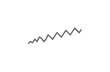
\begin{tikzpicture}[x=0.08em, y=0.08em, line width=0.4pt]
                \draw[FooterGray] (0,3) -- (1,4) -- (2,3.5) -- (3,5) -- (4,4) -- (5,6) -- (6,5.5) -- (7,4) -- (8,5) -- (9,7) -- (10,6) -- (11,5) -- (12,6.5) -- (13,8) -- (14,7) -- (15,6) -- (16,7.5) -- (17,9) -- (18,8) -- (19,7) -- (20,8.5) -- (21,10) -- (22,9) -- (23,8) -- (24,9.5);
            \end{tikzpicture}%
        }%
        \hskip0.5cm%
    }%
    \vskip6pt%
}

%=============================================================================
% PACKAGES
%=============================================================================
\usepackage[utf8]{inputenc}
\usepackage[T1]{fontenc}
\usepackage{amsmath, amssymb, amsthm}
\usepackage{mathtools}
\usepackage{bm}
\usepackage{tikz}
\usetikzlibrary{arrows.meta, positioning, shapes, calc, decorations.pathreplacing, shadings}
\usepackage{booktabs}
\usepackage{multirow}
\usepackage{array}
\usepackage{graphicx}
\usepackage{hyperref}
\usepackage{colortbl}
\hypersetup{colorlinks=true, linkcolor=MainBlue, urlcolor=MainBlue}
\graphicspath{{../../logos/}{../../charts/}{../../photos/}}
\hfuzz=2pt  % Suppress tiny overfull warnings (<2pt)
\vfuzz=2pt  % Suppress tiny vertical overfull warnings (<2pt)

%=============================================================================
% QUANTLET COMMAND
%=============================================================================
\newcommand{\quantlet}[2]{%
    \hfill\href{#2}{%
        \raisebox{-0.15em}{\includegraphics[height=0.7em]{ql_logo.png}}%
        \textcolor{MainBlue}{\tiny\ #1}%
    }%
}

%=============================================================================
% CUSTOM TITLE PAGE
%=============================================================================
\defbeamertemplate*{title page}{hybrid}[1][]
{
    \vspace{0.2cm}
    % Logos row - top header (with clickable links)
    \begin{center}
        \href{https://www.ase.ro}{\includegraphics[height=1.0cm]{ase_logo.png}}\hspace{0.3cm}%
        \href{https://theida.net}{\includegraphics[height=1.0cm]{ida_logo.png}}\hspace{0.3cm}%
        \href{https://blockchain-research-center.com}{\includegraphics[height=1.0cm]{brc_logo.png}}\hspace{0.3cm}%
        \href{https://www.ai4efin.ase.ro}{\includegraphics[height=1.0cm]{ai4efin_logo.png}}\hspace{0.3cm}%
        \href{https://ipe.ro/new}{\includegraphics[height=1.0cm]{acad_logo.png}}\hspace{0.3cm}%
        \href{https://www.digital-finance-msca.com}{\includegraphics[height=1.0cm]{msca_logo.png}}%
    \end{center}

    \vspace{0.6cm}

    % Main title with Q logos on sides (with clickable links)
    \begin{center}
        \begin{minipage}{0.1\textwidth}
            \centering
            \href{https://quantlet.com}{\includegraphics[height=1.1cm]{ql_logo.png}}
        \end{minipage}%
        \begin{minipage}{0.78\textwidth}
            \centering
            {\LARGE\bfseries\usebeamercolor[fg]{title}\inserttitle}

            \vspace{0.3cm}

            {\usebeamerfont{subtitle}\usebeamercolor[fg]{title}\insertsubtitle}
        \end{minipage}%
        \begin{minipage}{0.1\textwidth}
            \centering
            \href{https://quantinar.com}{\includegraphics[height=1.1cm]{qr_logo.png}}
        \end{minipage}
    \end{center}

    \vspace{0.6cm}

    % Authors (left aligned)
    \hspace{0.5cm}{\usebeamerfont{author}\insertauthor}

    \vspace{0.3cm}

    % Institute/Affiliations (left aligned)
    \hspace{0.5cm}\begin{minipage}[t]{0.9\textwidth}
        \raggedright\small\insertinstitute
    \end{minipage}
}

%=============================================================================
% THEOREM ENVIRONMENTS
%=============================================================================
\theoremstyle{definition}
\setbeamertemplate{theorems}[numbered]
\newtheorem{defn}{Definition}
\newtheorem{thm}{Theorem}
\newtheorem{prop}{Proposition}
\newtheorem{rmk}{Remark}

%=============================================================================
% CUSTOM COMMANDS
%=============================================================================
\newcommand{\E}{\mathbb{E}}
\newcommand{\Var}{\text{Var}}
\newcommand{\Cov}{\text{Cov}}
\newcommand{\Corr}{\text{Corr}}
\newcommand{\R}{\mathbb{R}}
\newcommand{\N}{\mathbb{N}}
\newcommand{\Z}{\mathbb{Z}}
\newcommand{\B}{\mathbf{B}}
\newcommand{\imark}{\textcolor{MainBlue}{\textbullet}}
\newcommand{\RMSE}{\text{RMSE}}
\newcommand{\MAE}{\text{MAE}}
\newcommand{\MAPE}{\text{MAPE}}
% Bold vector/matrix commands
\newcommand{\bY}{\mathbf{Y}}
\newcommand{\bA}{\mathbf{A}}
\newcommand{\bPi}{\boldsymbol{\Pi}}
\newcommand{\bGamma}{\boldsymbol{\Gamma}}
\newcommand{\bbeta}{\boldsymbol{\beta}}
\newcommand{\balpha}{\boldsymbol{\alpha}}
\newcommand{\bepsilon}{\boldsymbol{\varepsilon}}

%=============================================================================
% CENTRED MINIPAGE (no extra vertical space)
%=============================================================================
\newenvironment{cminipage}[1]{%
    \par\noindent\hfill\begin{minipage}{#1}\ignorespaces
}{%
    \end{minipage}\hfill\null\par
}

%=============================================================================
% TITLE INFORMATION
%=============================================================================
\title[Time Series Analysis]{Time Series Analysis and Forecasting}
\subtitle{Chapter 7: Cointegration and VECM}
\author[D.T. Pele]{Daniel Traian PELE}
\institute{Bucharest University of Economic Studies\\
IDA Institute Digital Assets\\
Blockchain Research Center\\
AI4EFin Artificial Intelligence for Energy Finance\\
Romanian Academy, Institute for Economic Forecasting\\
MSCA Digital Finance}
\date{}

\begin{document}

% Title page (no header/footer)
{
\setbeamertemplate{headline}{}
\setbeamertemplate{footline}{}
\begin{frame}
    \titlepage
\end{frame}
}

%=============================================================================
% LEARNING OBJECTIVES
%=============================================================================
\begin{frame}{Learning Objectives}
    \vspace{-0.3cm}
    {\small
\begin{block}{By the end of this chapter, you will be able to:}
\begin{itemize}\setlength{\itemsep}{0pt}
    \item Understand the problem of spurious regression with non-stationary data
    \item Test for cointegration using Engle-Granger and Johansen methods
    \item Estimate Vector Error Correction Models (VECM)
    \item Interpret error correction mechanisms and adjustment speeds
\end{itemize}
\end{block}
    }
\end{frame}

%=============================================================================
% TABLE OF CONTENTS
%=============================================================================
\begin{frame}{Outline}
    \begin{cminipage}{0.95\textwidth}
    \tableofcontents
    \end{cminipage}
\end{frame}

\section{Motivation}
%=============================================================================

\begin{frame}{Why Cointegration Matters}
    \begin{cminipage}{0.95\textwidth}
    \vspace{-0.2cm}
    \begin{block}{The Challenge}
        \begin{itemize}\setlength{\itemsep}{0pt}
            \item Many economic/financial time series are \textbf{non-stationary} (I(1))
            \item GDP, stock prices, exchange rates, interest rates all have unit roots
            \item Standard regression with I(1) variables $\Rightarrow$ \textbf{spurious results}
            \item Differencing removes non-stationarity but loses \textbf{long-run information}
        \end{itemize}
    \end{block}

    \vspace{0.15cm}

    \begin{alertblock}{The Solution: Cointegration}
        Some non-stationary series share a \textbf{common stochastic trend}---they move together in the long run.
    \end{alertblock}

    \vspace{0.15cm}

    \begin{exampleblock}{Nobel Prize 2003}
        Granger \& Engle received the Nobel Prize for ``methods for analyzing economic time series with common trends.''
    \end{exampleblock}
    \end{cminipage}
\end{frame}

\begin{frame}{Real-World Applications}
    \begin{cminipage}{0.95\textwidth}
    \vspace{-0.3cm}
    {\small
    \begin{columns}[T]
        \begin{column}{0.48\textwidth}
            \begin{block}{Finance}
                \begin{itemize}\setlength{\itemsep}{0pt}
                    \item \textbf{Pairs Trading}: Cointegrated stocks
                    \item \textbf{Term Structure}: Interest rates
                    \item \textbf{Spot-Futures}: Arbitrage
                \end{itemize}
            \end{block}

            \vspace{0.1cm}

            \begin{block}{Macroeconomics}
                \begin{itemize}\setlength{\itemsep}{0pt}
                    \item \textbf{Consumption \& Income}
                    \item \textbf{Money \& Prices}
                    \item \textbf{PPP}: Exchange rates
                \end{itemize}
            \end{block}
        \end{column}
        \begin{column}{0.48\textwidth}
            \begin{block}{Policy Analysis}
                \begin{itemize}\setlength{\itemsep}{0pt}
                    \item \textbf{Fiscal}: Spending \& taxes
                    \item \textbf{Monetary}: Rate pass-through
                    \item \textbf{Labor}: Wages \& productivity
                \end{itemize}
            \end{block}
        \end{column}
    \end{columns}
    }
    \end{cminipage}
\end{frame}

%=============================================================================
\section{Spurious Regression}
%=============================================================================

\begin{frame}{Spurious Regression: Visual Example}
    \vspace{-0.2cm}
    {\scriptsize
    \begin{alertblock}{Warning}
        \begin{itemize}\setlength{\itemsep}{0pt}
            \item \textbf{Result}: Two completely independent random walks show high correlation ($R^2 > 0.8$) purely by chance! This is why we need cointegration analysis
        \end{itemize}
    \end{alertblock}
    }
    \begin{center}
        \includegraphics[width=0.95\textwidth, height=0.50\textheight, keepaspectratio]{spurious_regression.pdf}
    \end{center}
    \quantlet{TSA\_ch7\_spurious\_regression}{https://github.com/QuantLet/TSA/tree/main/TSA_ch7/TSA_ch7_spurious_regression}
\end{frame}

\begin{frame}{The Spurious Regression Problem}
    \begin{cminipage}{0.95\textwidth}
    \begin{block}{Granger \& Newbold (1974)}
        Regressing one random walk on another \textbf{independent} random walk:
        $Y_t = \alpha + \beta X_t + u_t$ where $Y_t$ and $X_t$ are independent I(1) processes.
    \end{block}

    \vspace{0.15cm}

    \begin{alertblock}{Symptoms of Spurious Regression}
        \begin{itemize}\setlength{\itemsep}{0pt}
            \item High $R^2$ (often $> 0.9$) even though variables are \textbf{unrelated}
            \item Highly significant $t$-statistics (reject $H_0: \beta = 0$)
            \item Very low Durbin-Watson statistic ($DW \approx 0$)
            \item Residuals are non-stationary (have unit root)
        \end{itemize}
    \end{alertblock}

    \vspace{0.1cm}

    \begin{exampleblock}{Rule of Thumb}
        If $R^2 > DW$, suspect spurious regression!
    \end{exampleblock}
    \end{cminipage}
\end{frame}

\begin{frame}{Spurious Correlations in the Real World}
    \begin{cminipage}{0.95\textwidth}
    \begin{block}{Data Mining Can Produce Meaningless Correlations}
        With enough variables and long time series, purely coincidental patterns emerge:
    \end{block}

    \vspace{0.15cm}

    \begin{itemize}
        \item Distance between Neptune and Uranus $\leftrightarrow$ SAP SE stock price (2002--2023)
        \item GMO corn use in South Dakota $\leftrightarrow$ Google searches for ``i cant even'' (2004--2023)
        \item \textit{Two and a Half Men} season ratings $\leftrightarrow$ Jet fuel used in Serbia (2006--2015)
        \item ``Its Wednesday my dudes'' meme popularity $\leftrightarrow$ Boeing stock price (2006--2023)
    \end{itemize}

    \vspace{0.15cm}

    \begin{alertblock}{Lesson}
        High correlation $\neq$ causation. Non-stationary series with common trends produce high $R^2$ by construction. Always test for stationarity and cointegration before interpreting regression results!
    \end{alertblock}

    \vspace{0.1cm}
    {\footnotesize
    \faIcon{globe} Explore more examples: \href{https://www.tylervigen.com/spurious-correlations}{\texttt{tylervigen.com/spurious-correlations}}
    }
    \end{cminipage}
\end{frame}

%=============================================================================
\section{Cointegration Concept}
%=============================================================================

\begin{frame}{Cointegration: Visual Example}
    \vspace{-0.2cm}
    {\scriptsize
    \begin{exampleblock}{Key Insight}
        \begin{itemize}\setlength{\itemsep}{0pt}
            \item \textbf{Cointegration}: Both series are I(1) and trend together, but their linear combination (spread) is stationary --- this is cointegration!
        \end{itemize}
    \end{exampleblock}
    }
    \begin{center}
        \includegraphics[width=0.95\textwidth, height=0.50\textheight, keepaspectratio]{cointegrated_series.pdf}
    \end{center}
    \quantlet{TSA\_ch7\_cointegrated\_series}{https://github.com/QuantLet/TSA/tree/main/TSA_ch7/TSA_ch7_cointegrated_series}
\end{frame}

\begin{frame}{Definition of Cointegration}
    \begin{cminipage}{0.95\textwidth}
    \vspace{-0.3cm}
    {\small
    \begin{defn}[Cointegration (Engle \& Granger, 1987)]
        Variables $Y_{1t}, Y_{2t}, \ldots, Y_{kt}$ are \textbf{cointegrated of order $(d,b)$}, written $CI(d,b)$, if:
        \begin{enumerate}\setlength{\itemsep}{0pt}
            \item All variables are integrated of order $d$: $Y_{it} \sim I(d)$
            \item There exists a linear combination $\bbeta' \bY_t = \beta_1 Y_{1t} + \cdots + \beta_k Y_{kt}$ that is integrated of order $(d-b)$, where $b > 0$
        \end{enumerate}
    \end{defn}

    \vspace{0.3cm}

    \begin{block}{Most Common Case: $CI(1,1)$}
        \begin{itemize}\setlength{\itemsep}{0pt}
            \item Variables are $I(1)$ (have unit roots)
            \item Linear combination is $I(0)$ (stationary)
            \item Vector $\bbeta = (\beta_1, \ldots, \beta_k)'$ is the \textbf{cointegrating vector}
        \end{itemize}
    \end{block}

    \vspace{0.2cm}

    {\footnotesize
    The cointegrating vector is unique only up to scalar multiplication. Usually normalized: $\beta_1 = 1$.
    }
    }
    \end{cminipage}
\end{frame}

\begin{frame}{Intuition: Common Stochastic Trends}
    \begin{cminipage}{0.95\textwidth}
    \vspace{-0.2cm}
    {\small
    \begin{block}{Why Does Cointegration Occur?}
        Cointegrated variables share \textbf{common stochastic trends}:
        $Y_{1t} = \gamma_1 \tau_t + S_{1t}$, $Y_{2t} = \gamma_2 \tau_t + S_{2t}$
        where $\tau_t$ is a common random walk and $S_{it}$ are stationary.
    \end{block}

    \vspace{0.1cm}

    \begin{exampleblock}{Linear Combination Eliminates the Trend}
        $\gamma_2 Y_{1t} - \gamma_1 Y_{2t} = \gamma_2 S_{1t} - \gamma_1 S_{2t} \sim I(0)$
    \end{exampleblock}

    \vspace{0.1cm}

    \begin{alertblock}{Economic Interpretation}
        \begin{itemize}\setlength{\itemsep}{0pt}
            \item Cointegration = \textbf{long-run equilibrium relationship}
            \item Variables may deviate in the short run, but are ``pulled back''
            \item The cointegrating vector defines the equilibrium
        \end{itemize}
    \end{alertblock}
    }
    \end{cminipage}
\end{frame}

\begin{frame}{Cointegrating Rank}
    \begin{cminipage}{0.95\textwidth}
    \vspace{-0.2cm}
    {\small
    \begin{block}{How Many Cointegrating Relationships?}
        For $k$ variables that are $I(1)$:
        \begin{itemize}\setlength{\itemsep}{0pt}
            \item Maximum possible cointegrating relationships: $r = k - 1$
            \item If $r = 0$: No cointegration (variables drift apart)
            \item If $r = k$: All variables are $I(0)$ (contradiction)
        \end{itemize}
    \end{block}

    \vspace{0.3cm}

    \begin{exampleblock}{Example: 3 Variables}
        \begin{itemize}\setlength{\itemsep}{0pt}
            \item $r = 0$: No cointegration
            \item $r = 1$: One cointegrating relationship
            \item $r = 2$: Two cointegrating relationships (only 1 common trend)
        \end{itemize}
    \end{exampleblock}

    \vspace{0.2cm}

    {\footnotesize
    The number of common stochastic trends = $k - r$
    }
    }
    \end{cminipage}
\end{frame}

%=============================================================================
\section{Engle-Granger Method}
%=============================================================================

\begin{frame}{Engle-Granger Two-Step Method}
    \begin{cminipage}{0.95\textwidth}
    \vspace{-0.3cm}
    {\scriptsize
    \begin{block}{Step 1: Estimate Cointegrating Regression}
        Run OLS: $Y_t = \alpha + \beta X_t + e_t$. Save residuals: $\hat{e}_t = Y_t - \hat{\alpha} - \hat{\beta} X_t$
    \end{block}

    \vspace{0.1cm}

    \begin{block}{Step 2: Test Residuals for Stationarity}
        Test if $\hat{e}_t$ is $I(0)$ using ADF: $\Delta \hat{e}_t = \rho \hat{e}_{t-1} + \sum_{j=1}^{p} \gamma_j \Delta \hat{e}_{t-j} + v_t$
        \begin{itemize}\setlength{\itemsep}{0pt}
            \item $H_0$: $\rho = 0$ (unit root $\Rightarrow$ no cointegration)
            \item $H_1$: $\rho < 0$ (stationary $\Rightarrow$ cointegration)
        \end{itemize}
    \end{block}

    \vspace{0.1cm}

    \begin{alertblock}{Important}
        Use \textbf{Engle-Granger critical values}, not standard ADF! (More negative because residuals are estimated)
    \end{alertblock}
    }
    \end{cminipage}
\end{frame}

\begin{frame}{Engle-Granger Critical Values}
    \begin{cminipage}{0.95\textwidth}
    \begin{block}{Critical Values for Cointegration Test}
        {\small
        \begin{center}
        \begin{tabular}{lccc}
            \toprule
            \textbf{Variables} & \textbf{1\%} & \textbf{5\%} & \textbf{10\%} \\
            \midrule
            2 & $-3.90$ & $-3.34$ & $-3.04$ \\
            3 & $-4.29$ & $-3.74$ & $-3.45$ \\
            4 & $-4.64$ & $-4.10$ & $-3.81$ \\
            5 & $-4.96$ & $-4.42$ & $-4.13$ \\
            \bottomrule
        \end{tabular}
        \end{center}
        }
        {\footnotesize MacKinnon (1991), $T = 100$}
    \end{block}

    \vspace{0.15cm}

    \begin{alertblock}{Limitations of Engle-Granger}
        \begin{itemize}\setlength{\itemsep}{0pt}
            \item Only tests for \textbf{one} cointegrating relationship
            \item Results depend on choice of dependent variable
            \item Small sample bias; cannot test hypotheses on cointegrating vector
        \end{itemize}
    \end{alertblock}
    \end{cminipage}
\end{frame}

%=============================================================================
\section{Johansen Method}
%=============================================================================

\begin{frame}{Researcher Spotlight: Søren Johansen}
    \vspace{-0.3cm}
    \begin{columns}[T]
        \begin{column}{0.28\textwidth}
            \centering
            \includegraphics[width=0.95\textwidth, height=0.38\textheight, keepaspectratio]{photo_soren_johansen.jpg}
            \\[0.15cm]
            {\footnotesize\textcolor{MediumGray}{*1939}}\\[0.05cm]
            \href{https://en.wikipedia.org/wiki/S\%C3\%B8ren_Johansen}{\faWikipediaW\ \textcolor{MainBlue}{\small Wikipedia}}
        \end{column}
        \begin{column}{0.70\textwidth}
            {\footnotesize
            \begin{block}{Biography}
                \begin{itemize}\setlength{\itemsep}{0pt}
                    \item Danish statistician and econometrician, Professor Emeritus at University of Copenhagen
                    \item Known for his rigorous mathematical approach to econometrics
                    \item Fellow of the Econometric Society; recipient of numerous honors in statistical science
                \end{itemize}
            \end{block}
            \begin{exampleblock}{Key Contributions}
                \begin{itemize}\setlength{\itemsep}{0pt}
                    \item \textbf{Johansen cointegration test} (1988, 1991) --- maximum likelihood approach to testing for multiple cointegrating vectors
                    \item \textbf{Trace and maximum eigenvalue} statistics for determining cointegration rank
                    \item \textbf{VECM estimation} --- linking cointegration with error correction models
                    \item Standard framework for multivariate cointegration analysis in economics and finance
                \end{itemize}
            \end{exampleblock}
            }
        \end{column}
    \end{columns}
\end{frame}

\begin{frame}{Johansen Cointegration Test}
    \begin{cminipage}{0.95\textwidth}
    \begin{block}{Advantages over Engle-Granger}
        \begin{itemize}\setlength{\itemsep}{0pt}
            \item Tests for \textbf{multiple} cointegrating relationships
            \item Maximum likelihood estimation (more efficient)
            \item Can test restrictions on cointegrating vectors
            \item Does not require choosing a dependent variable
        \end{itemize}
    \end{block}

    \vspace{0.3cm}

    \begin{block}{Starting Point: VAR in Levels}
        $$\bY_t = \mathbf{c} + \bA_1 \bY_{t-1} + \bA_2 \bY_{t-2} + \cdots + \bA_p \bY_{t-p} + \bepsilon_t$$
    \end{block}

    \vspace{0.2cm}

    Rewrite in \textbf{Vector Error Correction} form...
    \end{cminipage}
\end{frame}

\begin{frame}{VECM Representation}
    \begin{block}{Vector Error Correction Model}
        $\Delta \bY_t = \mathbf{c} + \bPi \bY_{t-1} + \sum_{j=1}^{p-1} \bGamma_j \Delta \bY_{t-j} + \bepsilon_t$
        \begin{itemize}\setlength{\itemsep}{0pt}
            \item $\bPi = \sum_i \bA_i - \mathbf{I}$ (long-run impact); $\bGamma_j$ (short-run dynamics)
        \end{itemize}
    \end{block}

    \vspace{0.15cm}

    \begin{alertblock}{Key Insight: Rank of $\bPi$}
        The \textbf{rank of $\bPi$} determines cointegration:
        \begin{itemize}\setlength{\itemsep}{0pt}
            \item $\text{rank}(\bPi) = 0$: No cointegration (VAR in differences)
            \item $\text{rank}(\bPi) = k$: All variables are $I(0)$ (VAR in levels)
            \item $0 < \text{rank}(\bPi) = r < k$: $r$ cointegrating vectors
        \end{itemize}
    \end{alertblock}
\end{frame}

\begin{frame}{Derivation: From VAR to VECM}
    \vspace{-0.3cm}
    {\scriptsize
    \begin{block}{Starting Point: VAR(p) in Levels}
        $$\bY_t = \bA_1\bY_{t-1} + \bA_2\bY_{t-2} + \cdots + \bA_p\bY_{t-p} + \bepsilon_t$$
    \end{block}

    \vspace{0.1cm}

    \begin{block}{Step 1: Subtract $\bY_{t-1}$ from Both Sides}
        $$\bY_t - \bY_{t-1} = \bA_1\bY_{t-1} + \bA_2\bY_{t-2} + \cdots + \bA_p\bY_{t-p} - \bY_{t-1} + \bepsilon_t$$

        $$\Delta\bY_t = (\bA_1 - \mathbf{I})\bY_{t-1} + \bA_2\bY_{t-2} + \cdots + \bA_p\bY_{t-p} + \bepsilon_t$$
    \end{block}

    \vspace{0.1cm}

    \begin{alertblock}{Goal}
        Rewrite so that all terms are either in \textbf{levels} ($\bY_{t-1}$) or \textbf{differences} ($\Delta\bY_{t-j}$).
    \end{alertblock}
    }
\end{frame}

\begin{frame}{Derivation: From VAR to VECM (cont.)}
    \vspace{-0.2cm}
    {\footnotesize
    \begin{block}{Step 2: Add and Subtract Terms Strategically}
        Add $\bA_2\bY_{t-1}$ and subtract $\bA_2\bY_{t-1}$:
        $\Delta\bY_t = (\bA_1 + \bA_2 - \mathbf{I})\bY_{t-1} - \bA_2(\bY_{t-1} - \bY_{t-2}) + \bA_3\bY_{t-3} + \cdots + \bepsilon_t$

        Continue adding $\bA_3\bY_{t-1}$, etc., until all lagged \textbf{levels} are collected in one term.
    \end{block}

    \begin{block}{Step 3: General Pattern}
        After algebraic manipulation: $\Delta\bY_t = \bPi\bY_{t-1} + \sum_{j=1}^{p-1}\bGamma_j\Delta\bY_{t-j} + \bepsilon_t$
    \end{block}

    \begin{alertblock}{The Key Matrices}
        $\boxed{\bPi = \sum_{i=1}^{p}\bA_i - \mathbf{I} = -(\mathbf{I} - \bA_1 - \bA_2 - \cdots - \bA_p)}$ \quad
        $\boxed{\bGamma_j = -\sum_{i=j+1}^{p}\bA_i \text{ for } j = 1, \ldots, p-1}$
    \end{alertblock}
    }
\end{frame}

\begin{frame}{Derivation: Verifying the $\bGamma_j$ Formula}
    \begin{cminipage}{0.95\textwidth}
    \vspace{-0.15cm}
    {\small
    \begin{block}{Example: VAR(2)}
        Starting from: $\bY_t = \bA_1\bY_{t-1} + \bA_2\bY_{t-2} + \bepsilon_t$

        \vspace{0.1cm}
        Subtract $\bY_{t-1}$:
        $$\Delta\bY_t = (\bA_1 - \mathbf{I})\bY_{t-1} + \bA_2\bY_{t-2} + \bepsilon_t$$

        Add and subtract $\bA_2\bY_{t-1}$:
        $$\Delta\bY_t = (\bA_1 + \bA_2 - \mathbf{I})\bY_{t-1} + \bA_2(\bY_{t-2} - \bY_{t-1}) + \bepsilon_t$$
        $$\Delta\bY_t = \underbrace{(\bA_1 + \bA_2 - \mathbf{I})}_{\bPi}\bY_{t-1} \underbrace{- \bA_2}_{\bGamma_1}\Delta\bY_{t-1} + \bepsilon_t$$
    \end{block}

    \vspace{0.1cm}

    \begin{exampleblock}{Verification}
        For VAR(2): $\bPi = \bA_1 + \bA_2 - \mathbf{I}$ and $\bGamma_1 = -\bA_2$

        Using our formula: $\bGamma_1 = -\sum_{i=2}^{2}\bA_i = -\bA_2$ \quad $\checkmark$
    \end{exampleblock}
    }
    \end{cminipage}
\end{frame}

\begin{frame}{Economic Interpretation of Error Correction}
    \begin{cminipage}{0.95\textwidth}
    \begin{block}{The VECM with Cointegration}
        When $\text{rank}(\bPi) = r$, we write $\bPi = \balpha\bbeta'$:
        $\Delta\bY_t = \balpha\underbrace{(\bbeta'\bY_{t-1})}_{\text{equilibrium error}} + \sum_{j=1}^{p-1}\bGamma_j\Delta\bY_{t-j} + \bepsilon_t$
    \end{block}

    \begin{exampleblock}{Economic Interpretation}
        \begin{itemize}\setlength{\itemsep}{0pt}
            \item $\bbeta'\bY_{t-1}$ = \textbf{equilibrium error}: deviation from long-run relationship
            \item $\balpha$ = \textbf{adjustment speeds}: how fast variables correct deviations
            \item $\bGamma_j$ = \textbf{short-run dynamics}: transitory effects
        \end{itemize}
    \end{exampleblock}

    \begin{alertblock}{Error Correction Mechanism}
        If $\bbeta'\bY_{t-1} > 0$ (above equilibrium) and $\alpha_i < 0$, then $\Delta Y_{it}$ decreases.
        \textbf{The system self-corrects toward equilibrium!}
    \end{alertblock}
    \end{cminipage}
\end{frame}

\begin{frame}{Johansen Test Statistics}
    \vspace{-0.2cm}
    \begin{center}
        \includegraphics[width=0.95\textwidth, height=0.39\textheight, keepaspectratio]{johansen_eigenvalues.pdf}
    \end{center}
    \vspace{-0.2cm}
    {\scriptsize
    \begin{block}{When $\text{rank}(\bPi) = r < k$}
        $\bPi = \balpha \bbeta'$ where $\bbeta$ ($k \times r$) = \textbf{cointegrating vectors}, $\balpha$ ($k \times r$) = \textbf{adjustment coefficients}
    \end{block}

    \vspace{0.1cm}

    \begin{block}{Interpretation}
        \begin{itemize}\setlength{\itemsep}{0pt}
            \item $\bbeta' \bY_{t-1}$ = deviations from equilibrium (error correction terms)
            \item $\balpha$ = speed of adjustment; rows show each variable's response
        \end{itemize}
    \end{block}

    \vspace{0.1cm}

    {\scriptsize
    VECM: $\Delta \bY_t = \mathbf{c} + \balpha(\bbeta' \bY_{t-1}) + \sum_{j=1}^{p-1} \bGamma_j \Delta \bY_{t-j} + \bepsilon_t$
    }
    }
    \quantlet{TSA\_ch7\_johansen\_eigenvalues}{https://github.com/QuantLet/TSA/tree/main/TSA_ch7/TSA_ch7_johansen_eigenvalues}
\end{frame}

\begin{frame}{Testing Procedure}
    \begin{cminipage}{0.95\textwidth}
    \vspace{-0.3cm}
    {\footnotesize
    \begin{block}{Sequential Testing (Trace Test)}
        \begin{enumerate}\setlength{\itemsep}{0pt}
            \item Test $H_0$: $r = 0$. If rejected $\Rightarrow$ continue
            \item Test $H_0$: $r \leq 1$. If not rejected $\Rightarrow$ $r = 1$
            \item Continue until $H_0$ is not rejected
        \end{enumerate}
    \end{block}

    \vspace{0.1cm}

    \begin{alertblock}{Deterministic Components}
        \begin{itemize}\setlength{\itemsep}{0pt}
            \item No constant, no trend (rarely used)
            \item Constant in cointegrating relation only
            \item \textbf{Constant in both} (most common)
            \item Constant + trend in cointegrating relation
        \end{itemize}
    \end{alertblock}
    }
    \end{cminipage}
\end{frame}

%=============================================================================
\section{VECM Estimation}
%=============================================================================

\begin{frame}{Error Correction Mechanism: Visual}
    \vspace{-0.2cm}
    {\scriptsize
    \begin{block}{Interpretation}
        \begin{itemize}\setlength{\itemsep}{0pt}
            \item \textbf{Error correction}: When series deviate from equilibrium (shaded regions), the adjustment mechanism pulls them back. Positive deviations lead to downward adjustment, negative deviations lead to upward adjustment
        \end{itemize}
    \end{block}
    }
    \begin{center}
        \includegraphics[width=0.95\textwidth, height=0.50\textheight, keepaspectratio]{error_correction.pdf}
    \end{center}
    \quantlet{TSA\_ch7\_error\_correction}{https://github.com/QuantLet/TSA/tree/main/TSA_ch7/TSA_ch7_error_correction}
\end{frame}

\begin{frame}{VECM Structure}
    \begin{cminipage}{0.95\textwidth}
    \begin{block}{Full VECM Specification}
        For $k = 2$ variables with $r = 1$ cointegrating relation:
        \begin{align*}
            \Delta Y_{1t} &= c_1 + \alpha_1 (Y_{1,t-1} - \beta Y_{2,t-1}) + \gamma_{11} \Delta Y_{1,t-1} + \gamma_{12} \Delta Y_{2,t-1} + \varepsilon_{1t} \\
            \Delta Y_{2t} &= c_2 + \alpha_2 (Y_{1,t-1} - \beta Y_{2,t-1}) + \gamma_{21} \Delta Y_{1,t-1} + \gamma_{22} \Delta Y_{2,t-1} + \varepsilon_{2t}
        \end{align*}
    \end{block}

    \vspace{0.2cm}

    \begin{exampleblock}{Components}
        \begin{itemize}\setlength{\itemsep}{0pt}
            \item $(Y_{1,t-1} - \beta Y_{2,t-1})$ = error correction term (deviation from equilibrium)
            \item $\alpha_1, \alpha_2$ = adjustment speeds (should have opposite signs)
            \item $\gamma_{ij}$ = short-run dynamics
            \item $\varepsilon_{it}$ = innovations
        \end{itemize}
    \end{exampleblock}
    \end{cminipage}
\end{frame}

\begin{frame}{Interpreting Adjustment Coefficients}
    \begin{cminipage}{0.95\textwidth}
    \vspace{-0.2cm}
    \begin{block}{The $\alpha$ Coefficients}
        If the cointegrating relation is $Y_1 - \beta Y_2 = 0$ (equilibrium):

        \vspace{0.2cm}

        \begin{itemize}\setlength{\itemsep}{0pt}
            \item $\alpha_1 < 0$: $Y_1$ adjusts downward when above equilibrium
            \item $\alpha_2 > 0$: $Y_2$ adjusts upward when $Y_1$ is above equilibrium
        \end{itemize}
    \end{block}

    \vspace{0.3cm}

    \begin{alertblock}{Weak Exogeneity}
        If $\alpha_i = 0$, variable $Y_i$ does \textbf{not} respond to disequilibrium.
        \begin{itemize}\setlength{\itemsep}{0pt}
            \item $Y_i$ is \textbf{weakly exogenous} for the long-run parameters
            \item The other variable does all the adjusting
            \item Can simplify estimation (single-equation approach)
        \end{itemize}
    \end{alertblock}

    \vspace{0.2cm}

    {\footnotesize
    Test weak exogeneity: $H_0: \alpha_i = 0$ using likelihood ratio test.
    }
    \end{cminipage}
\end{frame}

\begin{frame}{VECM Impulse Response Functions}
    \vspace{-0.2cm}
    {\scriptsize
    \begin{block}{IRF Interpretation}
        \begin{itemize}\setlength{\itemsep}{0pt}
            \item \textbf{Permanent effects}: In a cointegrated system, shocks have permanent effects on levels, but the system returns to equilibrium --- they converge to a new long-run value
        \end{itemize}
    \end{block}
    }
    \begin{center}
        \includegraphics[width=0.95\textwidth, height=0.50\textheight, keepaspectratio]{vecm_irf.pdf}
    \end{center}
    \quantlet{TSA\_ch7\_vecm\_irf}{https://github.com/QuantLet/TSA/tree/main/TSA_ch7/TSA_ch7_vecm_irf}
\end{frame}

\begin{frame}{VECM vs VAR in Differences}
    \begin{cminipage}{0.95\textwidth}
    \vspace{-0.15cm}
    \begin{block}{When Variables are Cointegrated}
        \begin{center}
        \begin{tabular}{lcc}
            \toprule
            & \textbf{VAR in Differences} & \textbf{VECM} \\
            \midrule
            Long-run info & Lost & Preserved \\
            Short-run dynamics & Yes & Yes \\
            Error correction & No & Yes \\
            Forecasting & Poor (long-run) & Better \\
            IRF interpretation & Short-run only & Both \\
            \bottomrule
        \end{tabular}
        \end{center}
    \end{block}

    \vspace{0.3cm}

    \begin{alertblock}{Granger Representation Theorem}
        If variables are cointegrated, there \textbf{must} exist an error correction representation. Ignoring cointegration = model misspecification!
    \end{alertblock}
    \end{cminipage}
\end{frame}

%=============================================================================
\section{Practical Considerations}
%=============================================================================

\begin{frame}{Practical Workflow}
    \begin{cminipage}{0.95\textwidth}
    \begin{block}{Step-by-Step Procedure}
        \begin{enumerate}
            \item \textbf{Unit Root Tests}: Verify all variables are $I(1)$
            \begin{itemize}
                \item ADF, KPSS on levels and first differences
            \end{itemize}
            \item \textbf{Lag Length Selection}: Choose $p$ for VAR in levels
            \begin{itemize}
                \item Use AIC, BIC, or sequential LR tests
            \end{itemize}
            \item \textbf{Cointegration Test}: Johansen trace/max-eigenvalue tests
            \begin{itemize}
                \item Determine cointegrating rank $r$
            \end{itemize}
            \item \textbf{Estimate VECM}: If $0 < r < k$
            \begin{itemize}
                \item Estimate $\balpha$, $\bbeta$, $\bGamma_j$
            \end{itemize}
            \item \textbf{Diagnostics}: Check residuals for autocorrelation, normality
            \item \textbf{Analysis}: IRF, FEVD, hypothesis tests
        \end{enumerate}
    \end{block}
    \end{cminipage}
\end{frame}

\begin{frame}{Common Pitfalls}
    \begin{cminipage}{0.95\textwidth}
    \begin{alertblock}{Things to Watch Out For}
        \begin{itemize}\setlength{\itemsep}{0pt}
            \item \textbf{Structural breaks}: Cause spurious unit roots or cointegration
            \item \textbf{Near-unit-root}: Tests have low power
            \item \textbf{Lag selection}: Too many/few lags bias results
            \item \textbf{Small samples}: Johansen test oversized
        \end{itemize}
    \end{alertblock}

    \vspace{0.15cm}

    \begin{exampleblock}{Recommendation}
        Always check: residual diagnostics, stability of cointegrating relationship, sensitivity to specification
    \end{exampleblock}
    \end{cminipage}
\end{frame}

%=============================================================================
\section{Real-World Examples}
%=============================================================================

\begin{frame}{Example 1: Term Structure of Interest Rates}
    \vspace{-0.2cm}
    {\scriptsize
    \begin{exampleblock}{Expectations Hypothesis}
        \begin{itemize}\setlength{\itemsep}{0pt}
            \item \textbf{Conclusion}: Short and long rates share a common trend. The spread (term premium) is stationary --- evidence of cointegration!
        \end{itemize}
    \end{exampleblock}
    }
    \begin{center}
        \includegraphics[width=0.95\textwidth, height=0.50\textheight, keepaspectratio]{interest_rates_coint.pdf}
    \end{center}
    \quantlet{TSA\_ch7\_interest\_rates\_coint}{https://github.com/QuantLet/TSA/tree/main/TSA_ch7/TSA_ch7_interest_rates_coint}
\end{frame}

\begin{frame}{Example 2: Pairs Trading in Finance}
    \vspace{-0.2cm}
    {\scriptsize
    \begin{exampleblock}{Strategy}
        \begin{itemize}\setlength{\itemsep}{0pt}
            \item \textbf{Pairs trading}: Find cointegrated stock pairs (e.g., Coca-Cola \& Pepsi). When the spread deviates from the mean, trade expecting mean reversion
        \end{itemize}
    \end{exampleblock}
    }
    \begin{center}
        \includegraphics[width=0.95\textwidth, height=0.50\textheight, keepaspectratio]{pairs_trading.pdf}
    \end{center}
    \quantlet{TSA\_ch7\_pairs\_trading}{https://github.com/QuantLet/TSA/tree/main/TSA_ch7/TSA_ch7_pairs_trading}
\end{frame}

\begin{frame}{Interest Rates: Economic Theory}
    \begin{cminipage}{0.95\textwidth}
    \begin{block}{Expectations Hypothesis of the Term Structure}
        \begin{itemize}\setlength{\itemsep}{0pt}
            \item \textbf{Formula}: Long-term rate as average of expected future rates
            \begin{itemize}\setlength{\itemsep}{0pt}
                \item $R_t^{(n)} = \frac{1}{n} \sum_{i=0}^{n-1} E_t[r_{t+i}] + \text{term premium}$
            \end{itemize}
            \item \textbf{Implication}: If the term premium is constant, $r_t$ and $R_t$ are cointegrated
            \begin{itemize}\setlength{\itemsep}{0pt}
                \item Cointegrating vector: $(1, -1)$
            \end{itemize}
        \end{itemize}
    \end{block}

    \vspace{0.2cm}

    \begin{exampleblock}{Empirical Results}
        \begin{itemize}\setlength{\itemsep}{0pt}
            \item \textbf{Unit root tests}: Both rates are $I(1)$
            \begin{itemize}\setlength{\itemsep}{0pt}
                \item One cointegrating relationship (Johansen test)
            \end{itemize}
            \item \textbf{Cointegrating vector}: $\approx (1, -1)$, the spread is stationary
            \begin{itemize}\setlength{\itemsep}{0pt}
                \item The short rate adjusts to disequilibrium (the long rate is weakly exogenous)
            \end{itemize}
        \end{itemize}
    \end{exampleblock}
    \end{cminipage}
\end{frame}

\begin{frame}{Example 3: Purchasing Power Parity (PPP)}
    \vspace{-0.2cm}
    {\scriptsize
    \begin{block}{PPP Theory}
        \begin{itemize}\setlength{\itemsep}{0pt}
            \item \textbf{Formula}: $e_t = p_t - p_t^*$ (log exchange rate equals price differential). The real exchange rate should be stationary in the long run
        \end{itemize}
    \end{block}
    }
    \begin{center}
        \includegraphics[width=0.95\textwidth, height=0.50\textheight, keepaspectratio]{ppp_cointegration.pdf}
    \end{center}
    \quantlet{TSA\_ch7\_ppp\_cointegration}{https://github.com/QuantLet/TSA/tree/main/TSA_ch7/TSA_ch7_ppp_cointegration}
\end{frame}

\begin{frame}{VECM Results for Interest Rates}
    \begin{cminipage}{0.95\textwidth}
    \vspace{-0.15cm}
    \begin{block}{Typical Results}
        \begin{itemize}\setlength{\itemsep}{0pt}
            \item \textbf{Integration}: Both rates are $I(1)$, one cointegrating relationship identified
            \begin{itemize}\setlength{\itemsep}{0pt}
                \item Cointegrating vector close to $(1, -1)$: the spread is stationary
            \end{itemize}
            \item \textbf{Adjustment}: The short rate adjusts to the long rate
            \begin{itemize}\setlength{\itemsep}{0pt}
                \item The long rate does not adjust (weakly exogenous)
            \end{itemize}
        \end{itemize}
    \end{block}

    \begin{exampleblock}{VECM Equations (Stylized)}
        \begin{itemize}\setlength{\itemsep}{0pt}
            \item \textbf{Estimated system}:
            \begin{itemize}\setlength{\itemsep}{0pt}
                \item $\Delta r_t = 0.02 - 0.15(r_{t-1} - R_{t-1}) + \text{lags} + \varepsilon_{1t}$
                \item $\Delta R_t = 0.01 - 0.02(r_{t-1} - R_{t-1}) + \text{lags} + \varepsilon_{2t}$
            \end{itemize}
            \item \textbf{Interpretation}: The short rate adjusts faster ($\alpha_1 = -0.15$)
            \begin{itemize}\setlength{\itemsep}{0pt}
                \item The long rate is nearly weakly exogenous ($\alpha_2 \approx 0$)
            \end{itemize}
        \end{itemize}
    \end{exampleblock}
    \end{cminipage}
\end{frame}

%=============================================================================
\section{Case Study: Interest Rates}
%=============================================================================

\begin{frame}{Case Study: Cointegration of Interest Rates}
    \vspace{-0.2cm}
    {\scriptsize
    \begin{block}{Data}
        \begin{itemize}\setlength{\itemsep}{0pt}
            \item \textbf{US Interest Rates}: Long-term (10 years) and short-term (3 months)
            \item \textbf{Observation}: Both series are I(1), but the spread appears stationary
        \end{itemize}
    \end{block}
    }
    \begin{center}
        \includegraphics[width=0.95\textwidth, height=0.50\textheight, keepaspectratio]{ch7_case_raw_data.pdf}
    \end{center}
    \quantlet{TSA\_ch7\_case\_raw\_data}{https://github.com/QuantLet/TSA/tree/main/TSA_ch7/TSA_ch7_case_raw_data}
\end{frame}

\begin{frame}{Step 1: Unit Root Tests}
    \vspace{-0.2cm}
    {\scriptsize
    \begin{block}{Results}
        \begin{itemize}\setlength{\itemsep}{0pt}
            \item \textbf{ACF levels}: Slow decay --- non-stationarity; after differencing: rapid decay --- I(1)
            \item \textbf{ACF spread}: Stationary --- possible cointegration!
        \end{itemize}
    \end{block}
    }
    \begin{center}
        \includegraphics[width=0.95\textwidth, height=0.50\textheight, keepaspectratio]{ch7_case_unit_root.pdf}
    \end{center}
    \quantlet{TSA\_ch7\_case\_unit\_root}{https://github.com/QuantLet/TSA/tree/main/TSA_ch7/TSA_ch7_case_unit_root}
\end{frame}

\begin{frame}{Step 2: Engle-Granger Cointegration Test}
    \vspace{-0.2cm}
    {\scriptsize
    \begin{block}{Results}
        \begin{itemize}\setlength{\itemsep}{0pt}
            \item \textbf{Engle-Granger regression}: Short rate = $\alpha$ + $\beta$ $\times$ Long rate + $\varepsilon_t$
            \item \textbf{Conclusion}: The series are cointegrated --- a long-run equilibrium relationship exists
        \end{itemize}
    \end{block}
    }
    \begin{center}
        \includegraphics[width=0.95\textwidth, height=0.50\textheight, keepaspectratio]{ch7_case_cointegration.pdf}
    \end{center}
    \quantlet{TSA\_ch7\_case\_cointegration}{https://github.com/QuantLet/TSA/tree/main/TSA_ch7/TSA_ch7_case_cointegration}
\end{frame}

\begin{frame}{Step 3: VECM Estimation}
    \vspace{-0.2cm}
    {\scriptsize
    \begin{block}{Model}
        \begin{itemize}\setlength{\itemsep}{0pt}
            \item \textbf{VECM(2)}: Cointegration rank = 1
            \item \textbf{Adjustment}: The $\alpha$ coefficients indicate the speed of return to equilibrium
        \end{itemize}
    \end{block}
    }
    \begin{center}
        \includegraphics[width=0.95\textwidth, height=0.50\textheight, keepaspectratio]{ch7_case_vecm.pdf}
    \end{center}
    \quantlet{TSA\_ch7\_case\_vecm}{https://github.com/QuantLet/TSA/tree/main/TSA_ch7/TSA_ch7_case_vecm}
\end{frame}

\begin{frame}{Step 4: Impulse Response Functions}
    \vspace{-0.2cm}
    {\scriptsize
    \begin{block}{Interpretation}
        \begin{itemize}\setlength{\itemsep}{0pt}
            \item \textbf{Permanent effects}: Shocks to the long rate persistently affect both rates
            \item \textbf{Cointegration}: Effects do not converge to zero --- characteristic of cointegrated series
        \end{itemize}
    \end{block}
    }
    \begin{center}
        \includegraphics[width=0.95\textwidth, height=0.50\textheight, keepaspectratio]{ch7_case_irf.pdf}
    \end{center}
    \quantlet{TSA\_ch7\_case\_irf}{https://github.com/QuantLet/TSA/tree/main/TSA_ch7/TSA_ch7_case_irf}
\end{frame}

\begin{frame}{Step 5: VECM Forecast}
    \vspace{-0.2cm}
    {\scriptsize
    \begin{block}{Forecast}
        \begin{itemize}\setlength{\itemsep}{0pt}
            \item \textbf{Horizon}: 24 months for both rates simultaneously
            \item \textbf{Advantage}: VECM maintains the cointegrating relationship in the forecast
        \end{itemize}
    \end{block}
    }
    \begin{center}
        \includegraphics[width=0.95\textwidth, height=0.50\textheight, keepaspectratio]{ch7_case_forecast.pdf}
    \end{center}
    \quantlet{TSA\_ch7\_case\_forecast}{https://github.com/QuantLet/TSA/tree/main/TSA_ch7/TSA_ch7_case_forecast}
\end{frame}

%=============================================================================
\section{AI Use Case}
%=============================================================================

\begin{frame}{AI Exercise: Critical Thinking}
    \begin{cminipage}{0.95\textwidth}
    \vspace{-3mm}
    \begin{block}{\footnotesize Prompt to test in ChatGPT / Claude / Copilot}
        {\footnotesize
        ``Download daily prices for gold and silver using yfinance. Test for cointegration and estimate a VECM model. Analyze the speed of adjustment parameters. Give me complete Python code.''
        }
    \end{block}
    \vspace{-2mm}
    {\footnotesize
    \textbf{Exercise}:
    \begin{enumerate}\setlength{\itemsep}{0pt}
        \item Run the prompt in an LLM of your choice and critically analyze the response.
        \item Does it verify that each series is I(1) before testing for cointegration?
        \item Does it use both Engle-Granger and Johansen tests? What are the trade-offs?
        \item How does it determine the cointegration rank? Trace vs max-eigenvalue statistics?
        \item Does it correctly interpret the $\alpha$ (adjustment) coefficients?
    \end{enumerate}
    }
    \vspace{-2mm}
    \begin{alertblock}{}
        {\footnotesize \textbf{Warning}: AI-generated code may run without errors and look professional. \textit{That does not mean it is correct.}}
    \end{alertblock}
    \end{cminipage}
\end{frame}

%=============================================================================
\section{Summary}
%=============================================================================

\begin{frame}{Key Takeaways}
    \begin{cminipage}{0.95\textwidth}
    \vspace{-0.3cm}
    {\scriptsize
    \begin{block}{Main Concepts}
        \begin{itemize}\setlength{\itemsep}{0pt}
            \item \textbf{Cointegration}: $I(1)$ variables with stationary linear combination
            \item \textbf{Spurious regression}: High $R^2$ with unrelated $I(1)$ variables
            \item \textbf{VECM}: VAR with error correction for cointegrated systems
        \end{itemize}
    \end{block}

    \vspace{0.1cm}

    \begin{block}{Testing Methods}
        \begin{itemize}\setlength{\itemsep}{0pt}
            \item \textbf{Engle-Granger}: Simple, one vector only
            \item \textbf{Johansen}: Multiple vectors, MLE-based
        \end{itemize}
    \end{block}

    \vspace{0.1cm}

    \begin{alertblock}{Remember}
        Tests have low power in small samples. Theory should guide specification.
    \end{alertblock}
    }
    \end{cminipage}
\end{frame}

\begin{frame}{What's Next?}
    \begin{cminipage}{0.95\textwidth}
    \begin{block}{Extensions and Related Topics}
        \begin{itemize}\setlength{\itemsep}{0pt}
            \item \textbf{Structural VECM}: Identifying structural shocks
            \item \textbf{Threshold cointegration}: Nonlinear adjustment
            \item \textbf{Panel cointegration}: Multiple cross-sections
            \item \textbf{Fractional cointegration}: Long memory
            \item \textbf{Time-varying cointegration}: Regime changes
        \end{itemize}
    \end{block}

    \vspace{0.2cm}

    \begin{exampleblock}{}
        \begin{itemize}\setlength{\itemsep}{0pt}
            \item \textbf{Questions?}
        \end{itemize}
    \end{exampleblock}
    \end{cminipage}
\end{frame}

\begin{frame}{Key Formulas -- Summary}
    \vspace{-0.3cm}
    {\scriptsize
    \begin{columns}[T]
        \begin{column}{0.48\textwidth}
            \begin{block}{Cointegration}
                \begin{itemize}\setlength{\itemsep}{-1pt}
                    \item \textbf{Definition}: $Y_t - \beta X_t = u_t \sim I(0)$
                    \item \textbf{Interpretation}: Long-run equilibrium
                \end{itemize}
            \end{block}

            \begin{block}{Engle-Granger Test}
                \begin{itemize}\setlength{\itemsep}{-1pt}
                    \item \textbf{Step 1}: $Y_t = \alpha + \beta X_t + u_t$
                    \item \textbf{Step 2}: ADF test on $\hat{u}_t$
                    \item \textbf{Note}: Special critical values
                \end{itemize}
            \end{block}

            \begin{block}{Cointegration Rank}
                \begin{itemize}\setlength{\itemsep}{-1pt}
                    \item \textbf{Rank $r$}: $0 \leq r \leq K-1$ relationships
                \end{itemize}
            \end{block}
        \end{column}

        \begin{column}{0.48\textwidth}
            \begin{block}{VECM Model}
                \begin{itemize}\setlength{\itemsep}{-1pt}
                    \item \textbf{Equation}: $\Delta\bY_t = \bPi\bY_{t-1} + \sum_{i=1}^{p-1}\bGamma_i\Delta\bY_{t-i} + \bepsilon_t$
                    \item \textbf{Factorization}: $\bPi = \balpha\bbeta'$
                \end{itemize}
            \end{block}

            \begin{block}{Interpretation of $\balpha$ and $\bbeta$}
                \begin{itemize}\setlength{\itemsep}{-1pt}
                    \item \textbf{$\bbeta$}: Cointegrating vectors
                    \item \textbf{$\balpha$}: Speed of adjustment
                \end{itemize}
            \end{block}

            \begin{block}{Johansen Test}
                \begin{itemize}\setlength{\itemsep}{-1pt}
                    \item \textbf{Trace}: $\lambda_{trace} = -T\sum_{i=r+1}^{K}\ln(1-\hat{\lambda}_i)$
                    \item \textbf{Max-Eigen}: $\lambda_{max} = -T\ln(1-\hat{\lambda}_{r+1})$
                \end{itemize}
            \end{block}
        \end{column}
    \end{columns}
    }
\end{frame}

%=============================================================================
\section{Quiz}
%=============================================================================

\begin{frame}{Question 1}
    \begin{cminipage}{0.95\textwidth}
    \begin{alertblock}{Question}
        \begin{itemize}\setlength{\itemsep}{0pt}
            \item Analyze the two pairs of I(1) series below. Which pair is cointegrated?
        \end{itemize}
    \end{alertblock}

    \vspace{0.2cm}
    \begin{block}{Answer choices}
        \begin{enumerate}[(A)]\setlength{\itemsep}{0pt}
            \item Pair A, because the series have the same trend
            \item Pair B, because the series are uncorrelated
            \item Pair A, because their spread is stationary
            \item Both pairs are cointegrated
        \end{enumerate}
    \end{block}
    \end{cminipage}
\end{frame}

\begin{frame}{Question 1: Answer}
    \begin{cminipage}{0.95\textwidth}
    \vspace{0.3cm}
    \begin{center}
        \includegraphics[width=0.85\textwidth, height=0.45\textheight, keepaspectratio]{ch7_quiz1_cointegration_concept.pdf}
    \end{center}
    \vspace{-0.1cm}
    \begin{exampleblock}{Correct answer: (C) Pair A -- stationary spread}
        \begin{itemize}\setlength{\itemsep}{0pt}
            \item Cointegration = stationary linear combination, not just correlation
            \item Pair B's spread is non-stationary $\rightarrow$ not cointegrated
        \end{itemize}
    \end{exampleblock}
    \quantlet{TSA\_ch7\_quiz1\_cointegration\_concept}{https://github.com/QuantLet/TSA/tree/main/TSA_ch7/TSA_ch7_quiz1_cointegration_concept}
    \end{cminipage}
\end{frame}

\begin{frame}{Question 2}
    \begin{cminipage}{0.95\textwidth}
    \begin{alertblock}{Question}
        \begin{itemize}\setlength{\itemsep}{0pt}
            \item Both regressions below have high $R^2$. How can you distinguish a spurious regression from a genuine one?
        \end{itemize}
    \end{alertblock}

    \vspace{0.2cm}
    \begin{block}{Answer choices}
        \begin{enumerate}[(A)]\setlength{\itemsep}{0pt}
            \item Cannot distinguish -- both have high $R^2$
            \item Test the residuals: stationary residuals = genuine cointegration
            \item Check the significance of the $\beta$ coefficient
            \item Compare $R^2$ values: higher = more real relationship
        \end{enumerate}
    \end{block}
    \end{cminipage}
\end{frame}

\begin{frame}{Question 2: Answer}
    \begin{cminipage}{0.95\textwidth}
    \vspace{0.3cm}
    \begin{center}
        \includegraphics[width=0.85\textwidth, height=0.45\textheight, keepaspectratio]{ch7_quiz2_spurious_regression.pdf}
    \end{center}
    \vspace{-0.1cm}
    \begin{exampleblock}{Correct answer: (B) Test the stationarity of residuals}
        \begin{itemize}\setlength{\itemsep}{0pt}
            \item Engle-Granger test: if OLS residuals are stationary (ADF), the relationship is genuine
            \item High $R^2$ does NOT imply a real relationship between $I(1)$ variables!
        \end{itemize}
    \end{exampleblock}
    \quantlet{TSA\_ch7\_quiz2\_spurious\_regression}{https://github.com/QuantLet/TSA/tree/main/TSA_ch7/TSA_ch7_quiz2_spurious_regression}
    \end{cminipage}
\end{frame}

\begin{frame}{Question 3}
    \begin{cminipage}{0.95\textwidth}
    \begin{alertblock}{Question}
        \begin{itemize}\setlength{\itemsep}{0pt}
            \item In which scenario is the long rate weakly exogenous (does not adjust to disequilibrium)?
        \end{itemize}
    \end{alertblock}

    \vspace{0.2cm}
    \begin{block}{Answer choices}
        \begin{enumerate}[(A)]\setlength{\itemsep}{0pt}
            \item Scenario A: $\alpha_1 = -0.15$, $\alpha_2 = 0.02$
            \item Scenario B: $\alpha_1 = -0.05$, $\alpha_2 = -0.08$
            \item Scenario C: $\alpha_1 = 0.00$, $\alpha_2 = 0.20$
            \item No scenario -- both variables must adjust
        \end{enumerate}
    \end{block}
    \end{cminipage}
\end{frame}

\begin{frame}{Question 3: Answer}
    \begin{cminipage}{0.95\textwidth}
    \vspace{0.3cm}
    \begin{center}
        \includegraphics[width=0.85\textwidth, height=0.45\textheight, keepaspectratio]{ch7_quiz3_error_correction.pdf}
    \end{center}
    \vspace{-0.1cm}
    \begin{exampleblock}{Correct answer: (C) Scenario C -- $\alpha_1 = 0$}
        \begin{itemize}\setlength{\itemsep}{0pt}
            \item $\alpha_1 = 0$: the long rate does not respond to disequilibrium (weakly exogenous)
            \item All adjustment is done by the short rate ($\alpha_2 = 0.20$)
        \end{itemize}
    \end{exampleblock}
    \quantlet{TSA\_ch7\_quiz3\_error\_correction}{https://github.com/QuantLet/TSA/tree/main/TSA_ch7/TSA_ch7_quiz3_error_correction}
    \end{cminipage}
\end{frame}

\begin{frame}{Question 4}
    \begin{cminipage}{0.95\textwidth}
    \begin{alertblock}{Question}
        \begin{itemize}\setlength{\itemsep}{0pt}
            \item Given the Johansen Trace test results for $K=3$ variables, what is the cointegrating rank?
        \end{itemize}
    \end{alertblock}

    \vspace{0.2cm}
    \begin{block}{Answer choices}
        \begin{enumerate}[(A)]\setlength{\itemsep}{0pt}
            \item $r = 0$ (no cointegrating relationships)
            \item $r = 1$ (one cointegrating relationship)
            \item $r = 2$ (two cointegrating relationships)
            \item $r = 3$ (fully stationary system)
        \end{enumerate}
    \end{block}
    \end{cminipage}
\end{frame}

\begin{frame}{Question 4: Answer}
    \begin{cminipage}{0.95\textwidth}
    \vspace{0.3cm}
    \begin{center}
        \includegraphics[width=0.85\textwidth, height=0.45\textheight, keepaspectratio]{ch7_quiz4_johansen_rank.pdf}
    \end{center}
    \vspace{-0.1cm}
    \begin{exampleblock}{Correct answer: (C) $r = 2$ cointegrating relationships}
        \begin{itemize}\setlength{\itemsep}{0pt}
            \item Reject $H_0: r=0$ (45.2 > 29.8) and $H_0: r \leq 1$ (18.7 > 15.5)
            \item Cannot reject $H_0: r \leq 2$ (3.1 < 3.8) $\rightarrow$ rank is $r = 2$
        \end{itemize}
    \end{exampleblock}
    \quantlet{TSA\_ch7\_quiz4\_johansen\_rank}{https://github.com/QuantLet/TSA/tree/main/TSA_ch7/TSA_ch7_quiz4_johansen_rank}
    \end{cminipage}
\end{frame}

\begin{frame}{Question 5}
    \begin{cminipage}{0.95\textwidth}
    \begin{alertblock}{Question}
        \begin{itemize}\setlength{\itemsep}{0pt}
            \item What is the main advantage of VECM over VAR in differences for forecasting?
        \end{itemize}
    \end{alertblock}

    \vspace{0.2cm}
    \begin{block}{Answer choices}
        \begin{enumerate}[(A)]\setlength{\itemsep}{0pt}
            \item VECM has fewer parameters to estimate
            \item VECM preserves the cointegrating relationship in long-run forecasts
            \item VAR in differences cannot produce forecasts
            \item No advantage -- both are equivalent
        \end{enumerate}
    \end{block}
    \end{cminipage}
\end{frame}

\begin{frame}{Question 5: Answer}
    \begin{cminipage}{0.95\textwidth}
    \vspace{0.3cm}
    \begin{center}
        \includegraphics[width=0.85\textwidth, height=0.45\textheight, keepaspectratio]{ch7_quiz5_vecm_forecast.pdf}
    \end{center}
    \vspace{-0.1cm}
    \begin{exampleblock}{Correct answer: (B) VECM preserves cointegration}
        \begin{itemize}\setlength{\itemsep}{0pt}
            \item VAR($\Delta$) loses the level relationship $\rightarrow$ spread diverges
            \item VECM incorporates long-run equilibrium $\rightarrow$ forecast stays coherent
        \end{itemize}
    \end{exampleblock}
    \quantlet{TSA\_ch7\_quiz5\_vecm\_forecast}{https://github.com/QuantLet/TSA/tree/main/TSA_ch7/TSA_ch7_quiz5_vecm_forecast}
    \end{cminipage}
\end{frame}

\begin{frame}{Bibliography I}
    \begin{block}{Fundamental Cointegration Papers}
        {\small
        \begin{itemize}
            \item Engle, R.F., \& Granger, C.W.J. (1987). Co-Integration and Error Correction: Representation, Estimation, and Testing, \textit{Econometrica}, 55(2), 251--276.
            \item Johansen, S. (1988). Statistical Analysis of Cointegration Vectors, \textit{Journal of Economic Dynamics and Control}, 12(2-3), 231--254.
            \item Johansen, S. (1991). Estimation and Hypothesis Testing of Cointegration Vectors in Gaussian Vector Autoregressive Models, \textit{Econometrica}, 59(6), 1551--1580.
        \end{itemize}
        }
    \end{block}

    \begin{exampleblock}{VECM and Cointegration Textbooks}
        {\small
        \begin{itemize}
            \item Juselius, K. (2006). \textit{The Cointegrated VAR Model: Methodology and Applications}, Oxford University Press.
            \item L\"{u}tkepohl, H. (2005). \textit{New Introduction to Multiple Time Series Analysis}, Springer.
        \end{itemize}
        }
    \end{exampleblock}
\end{frame}

\begin{frame}{Bibliography II}
    \begin{block}{Tests and Applications}
        {\small
        \begin{itemize}
            \item Phillips, P.C.B., \& Ouliaris, S. (1990). Asymptotic Properties of Residual Based Tests for Cointegration, \textit{Econometrica}, 58(1), 165--193.
            \item Hamilton, J.D. (1994). \textit{Time Series Analysis}, Princeton University Press.
            \item Banerjee, A., Dolado, J.J., Galbraith, J.W., \& Hendry, D.F. (1993). \textit{Co-Integration, Error-Correction, and the Econometric Analysis of Non-Stationary Data}, Oxford University Press.
        \end{itemize}
        }
    \end{block}

    \begin{exampleblock}{Online Resources and Code}
        {\small
        \begin{itemize}
            \item \textbf{Quantlet}: \url{https://quantlet.com} $\rightarrow$ Code repository for statistics
            \item \textbf{Quantinar}: \url{https://quantinar.com} $\rightarrow$ Learning platform for quantitative methods
            \item \textbf{GitHub TSA}: \url{https://github.com/QuantLet/TSA} $\rightarrow$ Python code for this course
        \end{itemize}
        }
    \end{exampleblock}
\end{frame}

\begin{frame}{}
    \centering
    \Huge\textcolor{MainBlue}{Thank You!}

    \vspace{1cm}

    \Large Questions?

    \vspace{0.8cm}

    \normalsize

    Course materials available at: \url{https://danpele.github.io/Time-Series-Analysis/}

    \vspace{0.2cm}

    \href{https://quantlet.com}{\raisebox{-0.15em}{\includegraphics[height=0.8em]{ql_logo.png}} Quantlet} \hspace{0.5cm}
    \href{https://quantinar.com}{\raisebox{-0.15em}{\includegraphics[height=0.8em]{qr_logo.png}} Quantinar}
\end{frame}

\end{document}